\documentclass[dvipdfmx,11pt]{beamer}
%----------------------------------------------------------------------------------%
% \usetheme[progressbar=frametitle]{Amsterdam}
\usepackage{/Users/admin/Documents/mytex/mysty}
%----------------------------------------------------------------------------------%
%Beamer色設定
%Red: https://note.cman.jp/color/base_color.cgi
%Black
\definecolor{AlmostBlack}{RGB}{38,38,38}
%Blue
\definecolor{UniBlue}{RGB}{0,150,200}
\definecolor{Navy}{RGB}{0,0,128}
\definecolor{DarkBlue}{RGB}{0,0,100}
\definecolor{lavender}{RGB}{230,230,255}
%Red
\definecolor{AlertOrange}{RGB}{255,76,0}
\definecolor{FireBrick}{RGB}{178,34,34}
\definecolor{OrengeRed}{RGB}{255,69,0}
\definecolor{mistyrose}{RGB}{255,228,225}
%Green
\definecolor{DarkGreen}{RGB}{0,90,0}
\definecolor{MyGreen}{RGB}{0,77,5}
\definecolor{LightGreen}{RGB}{229,255,204}
%背景
\mode<beamer>{
    \definecolor{BackGroundGray}{RGB}{250,250,250}
    \setbeamercolor{background canvas}{bg=BackGroundGray} % スライドモードのみ背景をわずかにグレーにする
}
%----------------------------------------------------------------------------------%
%beamercolorの設定
\setbeamercolor{normal text}{fg=AlmostBlack}%本文の色
% \setbeamercolor{alerted text}{fg=OrengeRed}%\alertの色
\setbeamercolor{alerted text}{fg=FireBrick}%\alertの色
\setbeamercolor{structure}{fg=Navy}%\structreの色
\setbeamercolor{block title}{fg=white,bg=Navy}%ブロックのタイトルカラー
\setbeamercolor{block body}{fg=black,bg=lavender}%ブロックの本体のカラー
\setbeamercolor{block title alerted}{fg=white,bg=FireBrick}%ブロックのタイトルカラー
\setbeamercolor{block body alerted}{fg=black,bg=mistyrose}%ブロックの本体のカラー
\setbeamercolor{block title example}{fg=white,bg=DarkGreen}%ブロックのタイトルカラー
\setbeamercolor{block body example}{fg=black,bg=LightGreen}%ブロックの本体のカラー
\setbeamercolor*{palette secondary}{use=structure,fg=white,bg=DarkBlue} %上部の色
%----------------------------------------------------------------------------------%
\setbeamertemplate{navigation symbols}{} %ナビゲーションをなくす
% \setbeamertemplate{navigation symbols}{\insertframenumber}
\setbeamertemplate{footline}[frame number]{}%ページ番号
\setbeamercolor{page number in head/foot}{fg=black, bg=black}%ページ番号の色
\setbeamerfont{page number in head/foot}{family=\ttfamily,size=\small}%ページ番号のフォント・大きさ
\setbeamertemplate{footline}[frame number]%フッターをなくす
\setbeamertemplate{page number in head/foot}[totalframenumber]
% \setlength\abovecaptionskip{-2pt}
%----------------------------------------------------------------------------------%
% appendix
\newcommand{\backupbegin}{
   \newcounter{framenumberappendix}
   \setcounter{framenumberappendix}{\value{framenumber}}
}
\newcommand{\backupend}{
   \addtocounter{framenumberappendix}{-\value{framenumber}}
   \addtocounter{framenumber}{\value{framenumberappendix}} 
}
%----------------------------------------------------------------------------------%
\makeatletter
\newcommand*{\bkmtranslateto}{\languagename}
\newcommand*{\bkmtranslate}[1]{%
  \ifcsname tr@@@\bkmtranslateto @#1\endcsname
    \csname tr@@@\bkmtranslateto @#1\endcsname
  \else
    #1%
  \fi
}
\pdfstringdefDisableCommands{\let\translate\bkmtranslate}
\makeatother
%----------------------------------------------------------------------------------%
%%% 和文用 %%%
\usepackage{bxdpx-beamer}% ナビゲーションシンボル
\usepackage{pxjahyper}
\usepackage{minijs}
%%% 和文用 ここまで %%%
%----------------------------------------------------------------------------------%
\usepackage{bookmark}
\usepackage{helvet}
\usepackage{ascmac}
\usepackage{graphicx}
\usepackage{fancybox}
\usepackage{tikz}
\usetikzlibrary{patterns}
\usepackage{enumerate}
\usepackage{tcolorbox}
\renewcommand{\kanjifamilydefault}{\gtdefault} % 既定をゴシック体に
\usepackage[deluxe,uplatex]{otf} % 日本語多ウェイト化
\renewcommand\thefootnote{*\arabic{footnote})}%脚注のスタイル
% \renewcommand{\baselinestretch}{1.5}%行間を調整
%----------------------------------------------------------------------------------%
\usefonttheme{professionalfonts}% 数式
% \usepackage{txfonts}
% \usepackage{lmodern}
% \usepackage{ccfonts,eulervm}
\setbeamerfont{title}{size=\Large} % タイトル文字サイズ
\setbeamerfont{author}{size=\normalsize} % タイトル文字サイズ
\setbeamerfont{institute}{size=\scriptsize} % 所属の文字サイズ
\setbeamerfont{date}{size=\scriptsize} % 日付の文字サイズ
\setbeamerfont{frametitle}{size=\large} % フレームタイトルの文字サイズ
\setbeamerfont{footnote}{size=\scriptsize} % 脚注の文字サイズを小さくする
\useinnertheme{circles} % 箇条書きをシンプルにする
% \setbeamertemplate{items}[default]
\setbeamertemplate{itemize items}[circle]
\setbeamertemplate{enumerate item}[default]
% \setbeamertemplate{background}[grid][step=10mm]%背景を方眼に
%----------------------------------------------------------------------------------%
\newcommand{\kakko}[1]{\left\{ {#1} \right\}}
% \newtcolorbox{mybox}{colback=pink!30!white, colframe=red!50}
\newtcolorbox{mybox}{colback=pink!30!white, colframe=FireBrick}
%----------------------------------------------------------------------------------%
\AtBeginSection[]{%各セクションごとに目次を生成
  \begin{frame}[plain]\frametitle{}
    \setbeamertemplate{section in toc}[sections numbered]
    \tableofcontents[currentsection]
  \end{frame}
}
%----------------------------------------------------------------------------------%
\title{Study on a further improvement of \\ Maurer's universal statistical test}
\subtitle{}
% \date{\today}
\date{February 13, 2020}
% \author{引間 泰成}
\author{引間 泰成}
% \institute{\inst{1} 京都大学大学院情報学研究科修士2回 \and \inst{2} 京都大学大学院情報学研究科}
\institute{京都大学大学院 情報学研究科 数理工学専攻 物理統計学分野}
% \institute{%
% 京都大学大学院情報学研究科修士2回
% }
%----------------------------------------------------------------------------------%
%----------------------------------------------------------------------------------%
%----------------------------------------------------------------------------------%
\begin{document}
%----------------------------------------------------------------------------------%
%----------------------------------------------------------------------------------%
%----------------------------------------------------------------------------------%
% \maketitle%表紙の生成
\begin{frame}[plain]\frametitle{}
\titlepage %表紙
\end{frame}
%----------------------------------------------------------------------------------%
% \begin{frame}[plain]{Today's Topic}%目次の生成
%   \setbeamertemplate{section in toc}[sections numbered]
%   \tableofcontents[hideallsubsections]
% \end{frame}
%----------------------------------------------------------------------------------%
% \section{Maurer's universal test}
%----------------------------------------------------------------------------------%
% \begin{frame}[t]\frametitle{背景}
% \fbox{乱数検定}
% \vspace{.5\baselineskip}
% \begin{itemize}\setlength{\itemsep}{0.5\baselineskip}
%   \item (擬似)乱数生成器から生成された``$0$''と``$1$''から成る数列が応用先で求められる性質を満たしているかを統計的仮説検定によって評価する一般的な枠組み
%   \item 広く知られている乱数検定ツールとして\structure{NIST SP 800-22}がある
%   \item 本研究では,NIST SP 800-22に含まれている\alert{Maurer's universal test}に基づく統計検定について扱う
% \end{itemize}
% %
% \vspace{\baselineskip}
% \fbox{Maurer's universal test}
% \vspace{.5\baselineskip}
% \begin{itemize}\setlength{\itemsep}{0.5\baselineskip}
%   \item 1992年 Maurer によって提案された手法
%   \item[$\to$] 1999年 Coron によって修正
%   \item エントロピーに基づく検定統計量を計算し検定を行う
% \end{itemize}
% %
% \end{frame}
%----------------------------------------------------------------------------------%
\begin{frame}[t]\frametitle{背景}
\fbox{乱数}
\vspace{.2\baselineskip}
\begin{itemize}\setlength{\itemsep}{0.2\baselineskip}
  \item ``$0$''と``$1$''から成る``ランダム''な数列であり,工学をはじめとする様々な分野で用いられる
  \item[$\to$] 物理乱数生成器や擬似乱数生成器によって生成
\end{itemize}
%
\vspace{.5\baselineskip}
\fbox{乱数検定}
\vspace{.2\baselineskip}
\begin{itemize}\setlength{\itemsep}{0.2\baselineskip}
  \item (擬似)乱数生成器から生成された数列が応用先で求められる\\乱数としての性質を満たしているかを,統計的仮説検定に\\よって評価する一般的な枠組み
  \item 有名な乱数検定ツールとして\structure{NIST SP 800-22}がある
  \item 本研究では,NIST SP 800-22に採用されている\alert{Maurer's universal test}に基づく統計検定について扱う
\end{itemize}
%
\vspace{.5\baselineskip}
\fbox{Maurer's universal test}
\vspace{.2\baselineskip}
\begin{itemize}\setlength{\itemsep}{0.2\baselineskip}
  \item Maurerによって提案(1992)され,Coronが修正(1999)
  % \item[$\to$] 1999年 Coron によって修正
  \item エントロピーに基づく検定統計量を計算し検定を行う
\end{itemize}
%
\end{frame}
%----------------------------------------------------------------------------------%
\begin{frame}[t]\frametitle{検定の流れ}
\begin{itemize}\setlength{\itemsep}{0.5\baselineskip}
  \item 検定対象の系列を$L$ビットごとのブロックに分割し,初めの$Q$ブロックを初期化用,残りの$K$ブロックを検定用に用いる
  % 第$k$番目のブロックを$b_k$で表す
  \item 第$k$番目のブロックを$b_k$で表し,各ブロックに対して「\structure{そのブロックと一致する直近のブロックとの長さ(何ブロック前にあるか)}」を表す変数を計算する:
  \begin{align*}
    % \label{eq:An}
    A_n := \left\{ \begin{array}{ll}
    n, \quad \mathrm{if} \quad b_{n-l} \neq b_n \quad \mathrm{for} \quad 1 \leq l \leq n-1, \\
    \min \{ l \in \mathbb{N} \mid l \geq 1, b_{n-l} = b_n \},\quad \mathrm{otherwise}.
    \end{array} \right.
  \end{align*}
  %
  \item 検定対象の系列$x^n$に対し,検定統計量を次式で計算する:
  \begin{align*}
    f_C(x^n) = \frac{1}{K}\sum_{n=Q+1}^{Q+K} g(A_n), \quad \left( g(m) = (\log_2\mathrm{e}) \sum_{k=1}^{m-1}\frac{1}{k} \right).
  \end{align*}
  %
  \item[$\to$] 算出した検定統計量が平均$\mu$,分散$\sigma^2$の正規分布に近似的に従っているとみなして,p値を計算する
  %
\end{itemize}
%
\end{frame}
%----------------------------------------------------------------------------------%
\begin{frame}[c]\frametitle{Highly sensitive test [Yamamoto \& Liu, 2016]}
\begin{itemize}\setlength{\itemsep}{0.5\baselineskip}
  \item Maurer's (Coron's) test を基にした統計検定
  \item 検定対象の系列$x^n$を次の規則によって\underline{フリップする}:
    \begin{align*}
      \mathrm{Pr}\{ \hat{x}_i = 0 \mid x_i = 0 \} = 1, \quad
      \mathrm{Pr}\{ \hat{x}_i = 1 \mid x_i = 1 \} = \alpha.
    \end{align*}
  \item[$\to$] 変換後の系列$\hat{x}^n$は\alert{``$1$''をとる確率が$\hat{q}=\frac{\alpha}{2}$}となる
\end{itemize}
\vspace{\baselineskip}
\fbox{Highly sensitive test における帰無仮説}
\vspace{.5\baselineskip}
\begin{itemize}\setlength{\itemsep}{0.25\baselineskip}  
  \item $\mathcal{H}_0$:「検定対象の系列は$\{0,1\}^n$上の一様分布に従って生成\\されたとみなせる」
  \item $\widetilde{\mathcal{H}}_0$:「フリップに用いる乱数は理想的である」
\end{itemize}
%
\begin{itemize}
  \item[$\to$] $\overline{\mathcal{H}}_0:=\mathcal{H}_0 \land \widetilde{\mathcal{H}}_0$:「\structure{変換後の系列は``$1$''をとる確率が$\hat{q}$である\\ような$\{0,1\}^n$上の分布から独立に生成されたとみなせる}」
\end{itemize}
\end{frame}
%----------------------------------------------------------------------------------%
\begin{frame}[c]\frametitle{本研究の目的}
\begin{itemize}\setlength{\itemsep}{.5\baselineskip}
  \item Highly sensitive test では,次式で定義されるp値を計算する:
  \begin{align*}
      % p = \mathrm{erfc} \left( \left| \frac{f_C(\hat{x}^n) - L \times H(0.5\alpha)}{\sqrt{2}  \sigma_C(0.5\alpha)} \right| \right).
      p = \mathrm{erfc} \left( \left| \frac{f_C(\hat{x}^n) - \structure{L \times H(\hat{q})}}{\sqrt{2} \times \alert{\sigma_C(\hat{q})}} \right| \right).
      %
      \begin{picture}(0,0)
        \put(-55,20){\structure{\text{期待値}}}
        \put(-55,-22){\alert{\text{標準偏差}}}
      \end{picture}
    \end{align*}
\end{itemize}
%
\small
\begin{itemize}
  \item[※] $\mathrm{erfc}$は相補誤差関数,$H$は2値エントロピー関数を表す
\end{itemize}
\normalsize
%
\vspace{.5\baselineskip}
% \doublebox{課題}
\fbox{既往研究の課題}
\vspace{.5\baselineskip}
\begin{itemize}\setlength{\itemsep}{.5\baselineskip}
  \item $\hat{q} \neq 0.5$における\alert{参照分布の分散$\sigma_C(\hat{q})^2$}が理論的に導出されておらず,擬似乱数を用いて算出された値が使われている
  \item[$\to$] 定数であるパラメータが正しく与えられておらず,\\検定の信頼性の観点から好ましいとは言えない
\end{itemize}
%
\vspace{.5\baselineskip}
% \begin{center}
% % $\downarrow$\par
% \vspace{.5\baselineskip}
% \textcolor{FireBrick}{任意の$\hat{q}$に対する参照分布の分散を理論的に導出する}
% \end{center}
\begin{mybox}
\centering
参照分布の分散を任意の$\hat{q}$に対して理論的に導出する
\end{mybox}
\end{frame}
%----------------------------------------------------------------------------------%
% \section{参照分布の分散の導出}
%----------------------------------------------------------------------------------%
%----------------------------------------------------------------------------------%
\begin{frame}[c]\frametitle{参照分布の分散}
% 帰無仮説の下で$Q\to\infty$としたとき,系列$\{A_k\}_{k=1}^{K}$は\textit{ergodic stationary}である.このとき,
\textcolor{MyGreen}{参照分布の分散}$\sigma_{C,\hat{q}}(K)^2:=\sigma_C(\hat{q})^2$は次のように与えられる:
%
% \scriptsize
\small
\begin{align*}\begin{split}
% \label{eq:variance}
  &\sigma_{C,\hat{q}}(K)^2  \\
  % =& \mathrm{Var} [f_C(\hat{x}^n)] \\
  % =& \mathrm{Var} \left[ \frac{1}{K} \sum_{n=Q+1}^{K+Q} g(A_n) \right] \\
  % =& \frac{1}{K^2} \left( \sum_{n=Q+1}^{K+Q} \mathrm{Var} [g(A_n)] + 2 \sum_{1 \leq i < j \leq K} \mathrm{Cov} [g(A_{Q+i}), g(A_{Q+j})] \right) \\
  =& \frac{1}{K^2} \left( K \times \structure{\mathrm{Var} [g(A_n)]} + 2\sum_{k=1}^{K-1}(K-k)\times \alert{\mathrm{Cov}[g(A_n),g(A_{n+k})]} \right).
\end{split}\end{align*}
\normalsize
%
% \vspace{.5\baselineskip}
\structure{分散}および\alert{共分散}はそれぞれ次のように与えられる:
\small
\begin{align*}
  \mathrm{Var}[g(A_n)] =& \sum_{i=1}^{\infty} \{ g(i) \}^2 \structure{\mathrm{Pr}[A_n=i]} - \{ L H(\hat{q}) \}^2 ,\\
  \mathrm{Cov}[g(A_n),g(A_{n+k})] =& \sum_{i,j\geq 1} g(i)g(j) \alert{\mathrm{Pr}[A_n=i, \, A_{n+k}=j]}- \left\{L H(\hat{q})\right\}^2.
\end{align*}
\normalsize
%
% \vspace{.5\baselineskip}
\begin{itemize}\setlength{\itemsep}{0.5\baselineskip}
  \item \structure{周辺分布}および\alert{同時分布}の導出が必要 (\underline{以下で導出}) 
  \item 以下では,$w_r := \hat{q}^r(1 - \hat{q})^{L-r}$とおく
\end{itemize}
%
\small
\begin{itemize}
  \item[※] $\hat{q}$は系列において``$1$''をとる確率
\end{itemize}
\normalsize
%
\end{frame}
%----------------------------------------------------------------------------------%
\begin{frame}[c]\frametitle{周辺分布の導出}
\vspace{.5\baselineskip}
事象$\mathcal{M}$を次のように定める:
\begin{align*}
  \mathcal{M} = \left< b_{n-i} = b_{n}, b_{n-i+1} \neq b_{n} ,\dots, b_{n-1} \neq b_{n}  \right>.
\end{align*}
各ブロックが独立同分布に従うとき,
\begin{align*}
  \mathrm{Pr}[A_n=i] = \sum_{r=0}^{L} \mathrm{Pr}[\mathcal{M} \mid \ell(b_n) = r] \times \mathrm{Pr} [\ell(b_n) = r].
\end{align*}
ここに,$\ell(b)$はブロック$b$における``$1$''の個数を表す.また,
%
\begin{align*}
  \mathrm{Pr}[\mathcal{M} \mid \ell(b_n) = r] &= w_r \times ( 1 - w_r )^{i-1},\\
  \mathrm{Pr} [\ell(b_n) = r] &= \binom{L}{r} w_r. 
\end{align*}
よって,周辺分布は次式で与えられる:
\begin{align*}\begin{split}
  \mathrm{Pr}[A_n=i] = \sum_{r=0}^{L} \binom{L}{r} w_r^2 (1-w_r)^{i-1}.
\end{split}\end{align*}
\end{frame}
%----------------------------------------------------------------------------------%
\begin{frame}[c]\frametitle{同時分布の導出($k+1 \leq j \leq k+i-1$の場合)}
\vspace{.5\baselineskip}
事象$e_3 (b,b^\prime)$を次のように定める:
%
\begin{align*}
\begin{split}
  e_3 (b,b^\prime) := 
  &\left< b_{n-i} = b , b_{n} = b , b_{n+k-j} = b^\prime , b_{n+k} = b^\prime \right> \\
  &\land \left< b_{n-i+1} \neq b, \dots, b_{n+k-j-1} \neq b \right> \\
  &\land \left< b_{n+k-j+1} \neq b, \dots, b_{n-1} \neq b \right> \\
  &\land \left< b_{n+k-j+1} \neq b^\prime, \dots, b_{n-1} \neq b^\prime \right> \\
  &\land \left< b_{n+1} \neq b^\prime , \dots, b_{n+k-1} \neq b^\prime \right>.
\end{split}
\end{align*}
%
事象$e_3(b,b^\prime)$が起こる確率は以下で与えられる:
%
\begin{align*}
\begin{split}
  &\mathrm{Pr} \left[ e_3(b, b^\prime) \right]\\
  =& w_{r_1}^2 w_{r_2}^2 
  (1-w_{r_1})^{i-j+k-1} 
  (1-w_{r_1}-w_{r_2})^{j-k-1}
  (1-w_{r_2})^{k-1}.
\end{split}
\end{align*}
%
\begin{figure}
\centering
  \begin{tikzpicture}
    \draw (-0.3,0)--(0,0);
    \draw (-0.3,0.6)--(0,0.6);
    \draw (0,0) rectangle (0.6,0.6);
    \filldraw [draw=black, fill=pink] (0.6,0) rectangle (0.6*2, 0.6) node (A) at (0.9,0.6) [above]{$b_{n-i}$};
    \filldraw [pattern = north east lines] (0.6*2, 0) rectangle (0.6*3, 0.6);
    \filldraw [pattern = north east lines] (0.6*3, 0) rectangle (0.6*4, 0.6);
    \filldraw [draw=black, fill=yellow] (0.6*4, 0) rectangle (0.6*5, 0.6) node (B) at (2.7,0.6) [above] {$b_{n+k-j}$};
    \filldraw [pattern = crosshatch] (0.6*5, 0) rectangle (0.6*6, 0.6);
    \filldraw [pattern = crosshatch] (0.6*6, 0) rectangle (0.6*7, 0.6);
    \filldraw [pattern = crosshatch] (0.6*7, 0) rectangle (0.6*8, 0.6);
    \filldraw [draw=black, fill=pink] (0.6*8, 0) rectangle (0.6*9, 0.6)node (AA) at (5.1,0.6)[above] {$b_n$};
    \filldraw [pattern = north east lines] (0.6*9, 0) rectangle (0.6*10, 0.6);
    \filldraw [pattern = north east lines] (0.6*10, 0) rectangle (0.6*11, 0.6);
    \filldraw [pattern = north east lines] (0.6*11, 0) rectangle (0.6*12, 0.6);
    \filldraw [pattern = north east lines] (0.6*12, 0) rectangle (0.6*13, 0.6);
    \filldraw [pattern = north east lines] (0.6*13, 0) rectangle (0.6*14, 0.6);
    \filldraw [draw=black, fill=yellow] (0.6*14, 0) rectangle (0.6*15, 0.6)node (BB) at (8.7,0.6)[above]{$b_{n+k}$};
    \draw (0.6*15, 0) rectangle (0.6*16, 0.6);
    \draw (0.6*16, 0)--(0.6*16.5, 0);
    \draw (0.6*16, 0.6)--(0.6*16.5, 0.6);
    %
    \draw[<->] (A) to[bend left=20] node [above] {\small \alert{一致}} (AA);
    \draw[<->] (B) to[bend left=15] node [above] {\small \alert{一致}} (BB);
  \end{tikzpicture}
  % \caption{The arrangement of blocks in the case of $k+1 \leq j \leq k+i-1$}
  \label{fig:case3}
\end{figure}
\end{frame}
%----------------------------------------------------------------------------------%
\begin{frame}[c]\frametitle{同時分布の導出}
%
したがって,求める同時分布は次のように表される:
% \scriptsize
\begin{align*}
\begin{split}
  &\mathrm{Pr} [A_n=i,\, A_{n+k}=j] \\
  =& \mathrm{Pr} \left[ \bigvee_{b \in \{0,1\}^L} \bigvee_{b^\prime \in \{0,1\}^L \setminus \{b\}}
  e_3(b,b^\prime) \right] \\
  %
  =&\sum_{b \in \{0,1\}^L} \sum_{b^\prime \in \{0,1\}^{L} \setminus \{ b \}} \mathrm{Pr} \left[ e_3(b,b^\prime) \right] \\
  %
  % =& \sum_{r_1=0}^{L} \sum_{b_1 \in B^L_{r_1}} \sum_{r_2=0}^{L} \sum_{b_2 \in B^L_{r_2} \setminus \{ b_1 \}} \mathrm{Pr} \left[ e_3(b_1,b_2) \right] \\
  %
  % =& \sum_{r_1=0}^{L} \sum_{r_2 \neq r_1} \sum_{b_1 \in B^L_{r_1}} \sum_{b_2 \in B^L_{r_2}} \mathrm{Pr} \left[e_3(b_1,b_2) \right] \\ 
  % %
  % &+ \sum_{r_1=0}^{L} \sum_{r_2 \in \{r_1\}} \sum_{b_1 \in B^L_{r_1}} \sum_{b_2 \in B^L_{r_1} \setminus \{ b_1 \}} \mathrm{Pr} \left[e_3(b_1,b_2) \right] \\
  %
  =& \sum_{r_1=0}^{L} \sum_{r_2 \neq r_1} \dbinom{L}{r_1} \dbinom{L}{r_2} \mathrm{Pr} \left[e_3(b,b^\prime) \right] \\
  %
  &+ \sum_{r_1=0}^{L}\sum_{r_2\in\{r_1\}} \dbinom{L}{r_1} \left\{ \dbinom{L}{r_1} -1 \right\} \mathrm{Pr} \left[e_3(b,b^\prime) \right].
\end{split}
\end{align*}
%
% \footnotesize
%
\begin{itemize}
  \item[$\to$] \structure{周辺分布}および\alert{同時分布}を\textcolor{MyGreen}{参照分布の分散$\sigma_{C,\hat{q}}(K)^2$}の式に\\代入することにより,求める参照分布の分散が得られる 
\end{itemize}
\end{frame}
%----------------------------------------------------------------------------------%
% \section{計算機実験}
%----------------------------------------------------------------------------------%
\begin{frame}[c]\frametitle{計算機実験1: $L=4$の場合}
% 導出した式により,$L=4$のときの参照分布の分散を計算する
\centering
\begin{figure}
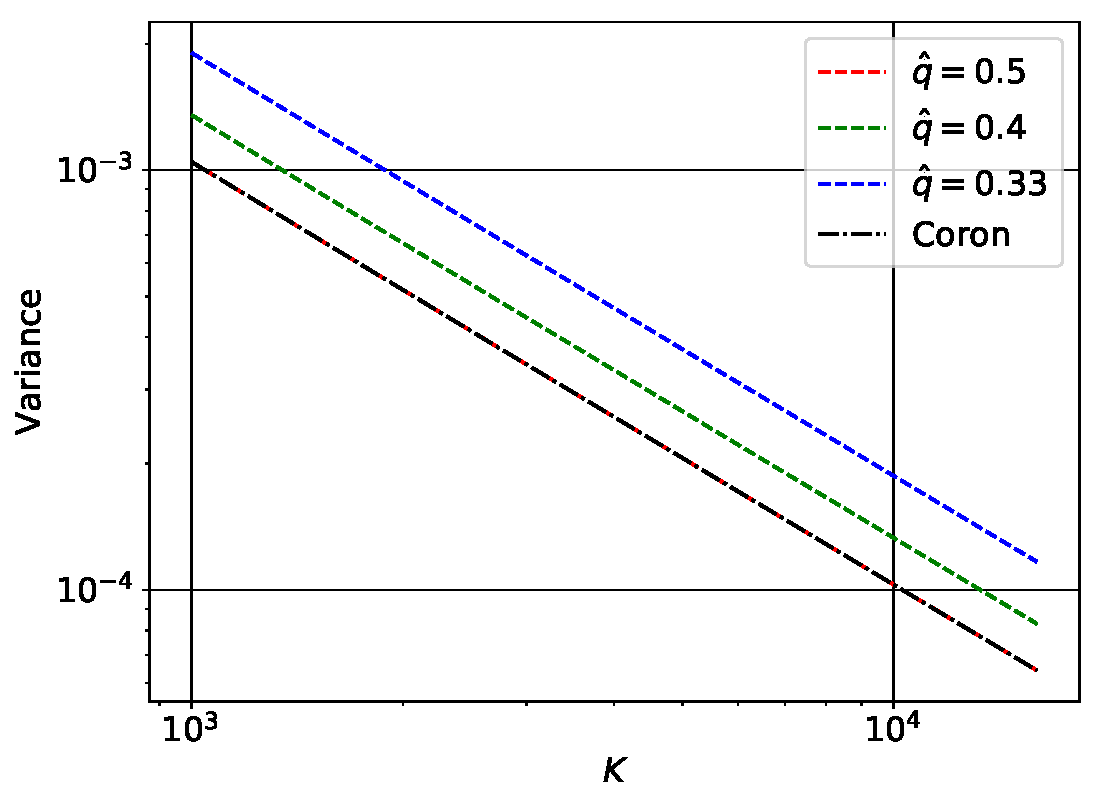
\includegraphics[width=.7\linewidth]{./figure/comparison_coron_L4_1000.pdf}
% \caption{}
\end{figure}
%
\begin{itemize}\setlength{\itemsep}{0.5\baselineskip}
  \item 参照分布の分散は$\mathcal{O}(\frac{1}{K})$で減少
  \item $\hat{q}=0.5$のとき,\underline{既往研究の結果と整合}
  \item 推奨値である$K=1000\times 2^4$における値が計算可能
\end{itemize}
%
\end{frame}
%----------------------------------------------------------------------------------%
\begin{frame}[c]\frametitle{計算機実験2: $L=8$の場合}
\begin{itemize}
  \item 計算が途中で破綻(左図)
  \item 次式による曲線近似を考える:
  \begin{align*}
  \sigma_{C,\hat{q}}^2 (K) = \frac{1}{K} \left( a + \frac{b}{K} \right),
\end{align*}
ここに,$a,b$は実数値定数.
\end{itemize}
%
%
\centering
% \begin{figure}
%    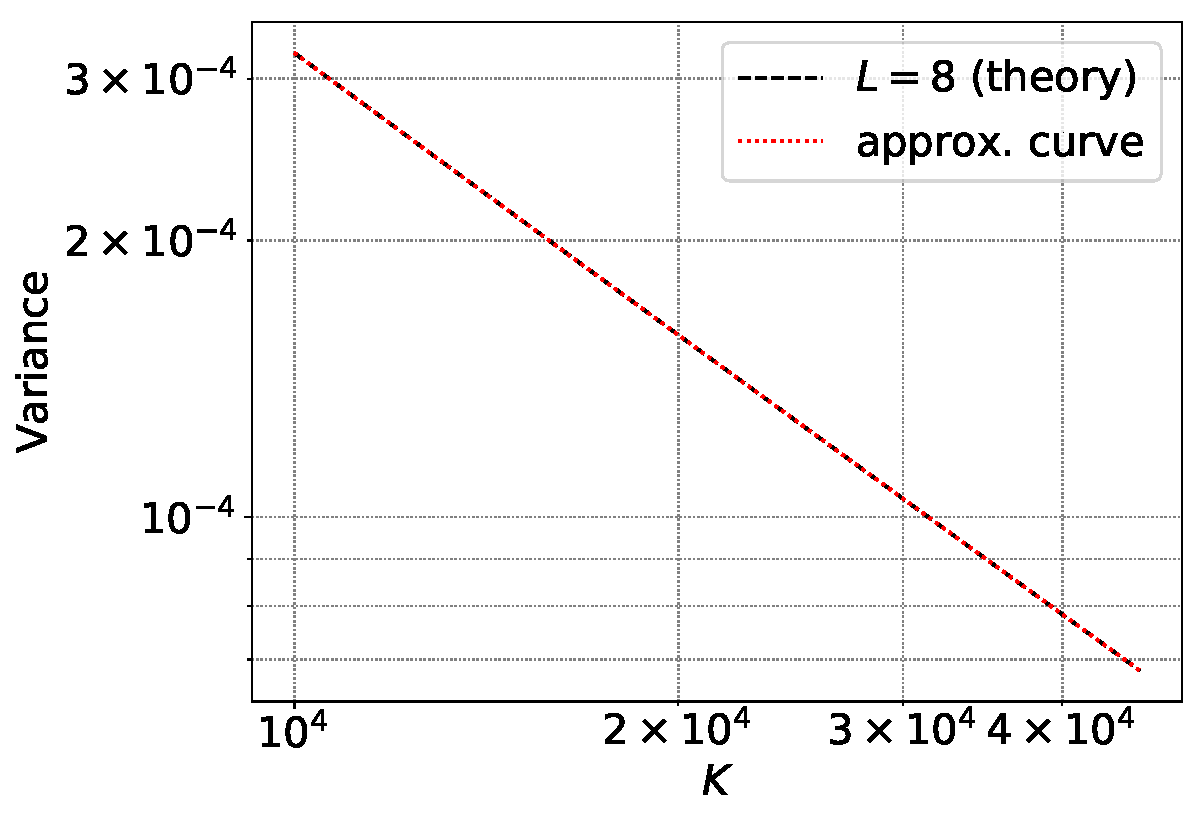
\includegraphics[width=.7\linewidth]{./figure/approx_varf_log_L8_10000.pdf}
%    % \caption{ほげ}
% \end{figure}
%
\begin{figure}[h]
 \begin{minipage}{0.49\hsize}
  \begin{center}
   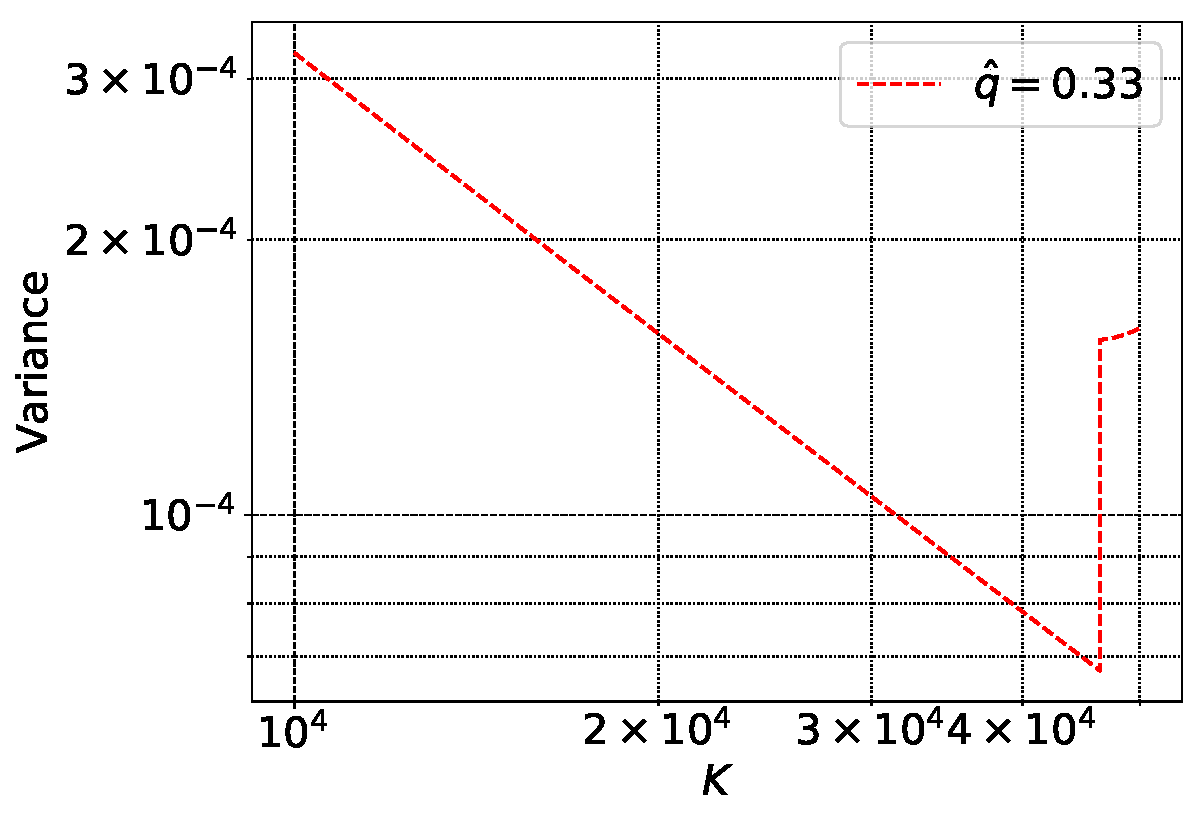
\includegraphics[width=.95\linewidth]{./figure/hatan.pdf}
  \end{center}
  % \caption{一つめの図}
  % \label{fig:one}
 \end{minipage}
 \begin{minipage}{0.49\hsize}
  \begin{center}
   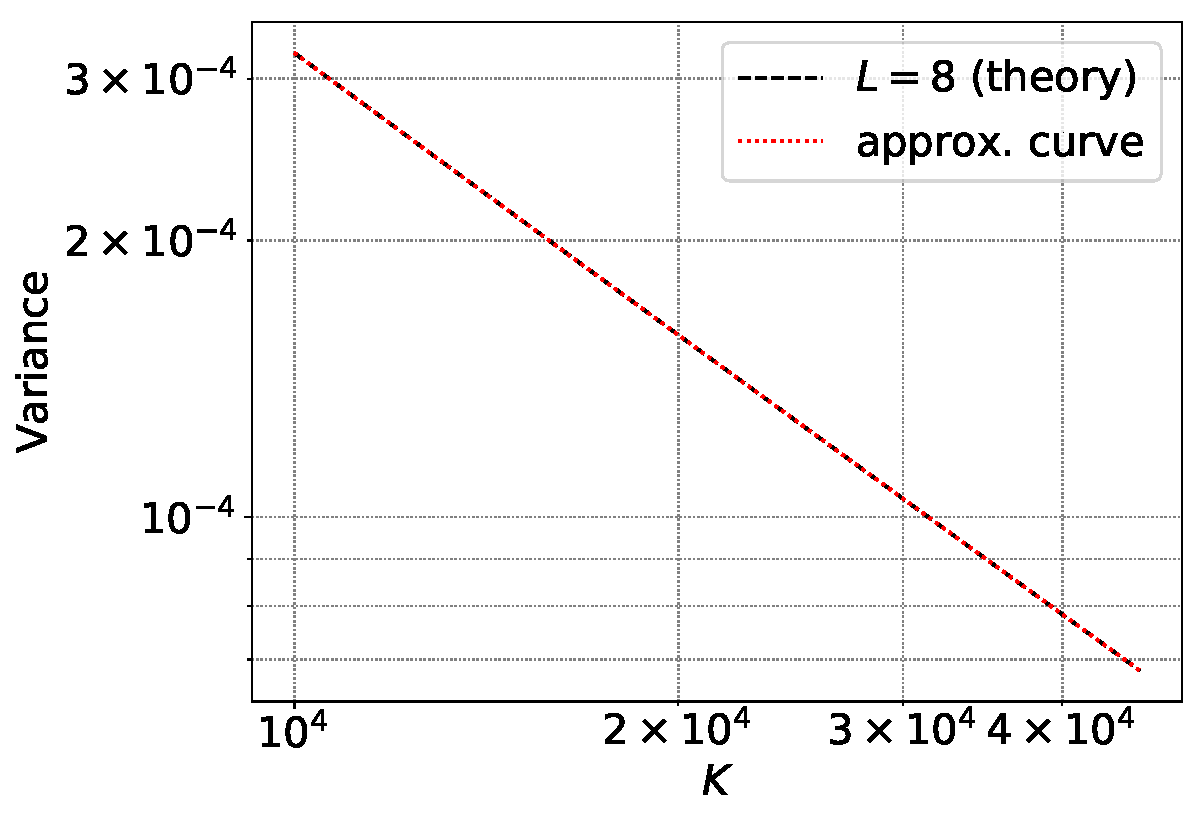
\includegraphics[width=.95\linewidth]{./figure/approx_varf_log_L8_10000.pdf}
  \end{center}
  % \caption{二つめの図}
  % \label{fig:two}
 \end{minipage}
\end{figure}
%
\begin{itemize}
  \item 近似曲線が理論的な値と整合している(右図)
  \item[$\to$] 推奨値: $K=1000\times 2^8$の値を算出
\end{itemize}
%
\end{frame}
%----------------------------------------------------------------------------------%
\begin{frame}[t]\frametitle{計算機実験3: 擬似乱数を用いて算出した値との比較}

\begin{table}[htb]
  \begin{tabular}{cccc} \hline
     & Yamamoto\&Liu & Proposed & \structure{MT} \\ \hline 
    $\sigma_{C,0.33}(K)$ & $\textcolor{FireBrick}{0.0034}9225$ & $\textcolor{FireBrick}{0.003488}60$ & $\textcolor{FireBrick}{0.003488}16$ \\ \hline
  \end{tabular}
\end{table}
%
\small
\begin{itemize}
  \item[※] \structure{MT}: Mersenne Twister を用いて算出した値(10回の試行の平均値)
\end{itemize}
\normalsize
%
\centering
\begin{figure}
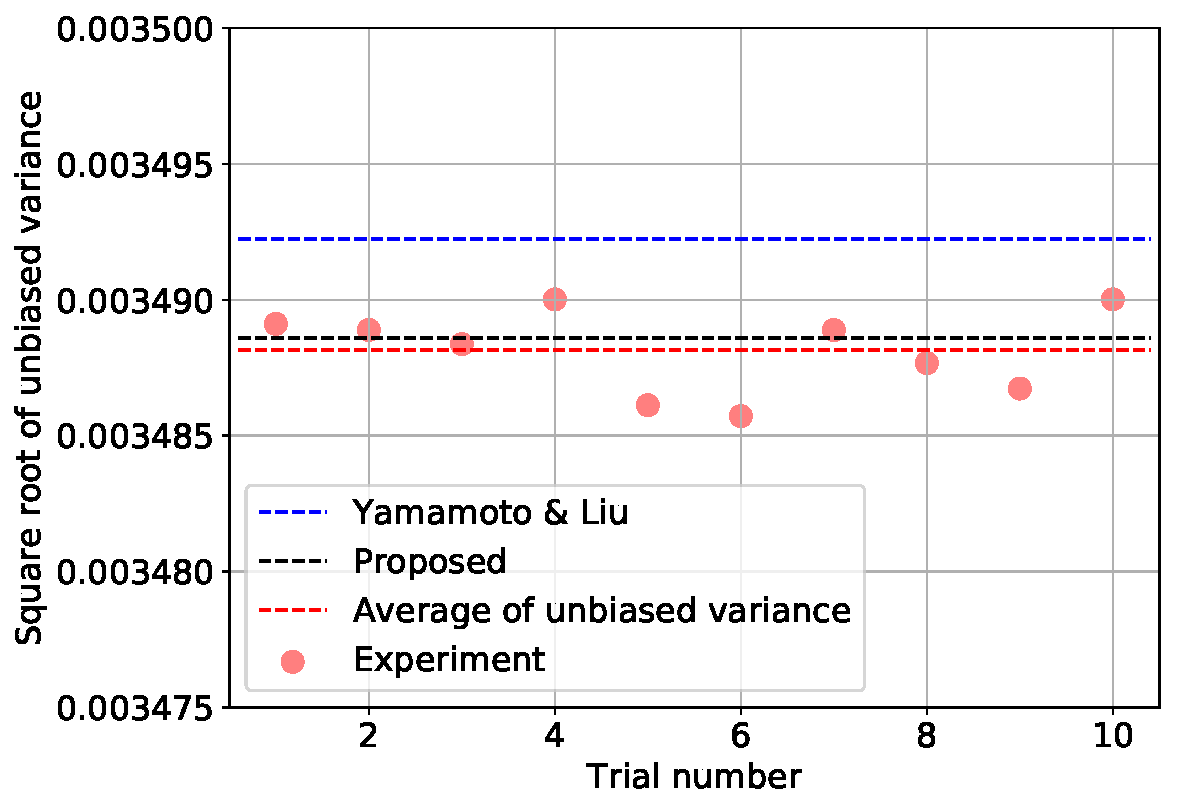
\includegraphics[width=.7\linewidth]{./figure/unbiased_variance.pdf}
% \caption{}
\end{figure}
%
\begin{center}
\structure{既往研究で与えられている数値}よりも\underline{実験結果と整合}
\end{center}
\end{frame}
%----------------------------------------------------------------------------------%
\begin{frame}[c]\frametitle{まとめ}
    
% まとめ:
\vspace{.5\baselineskip}
\begin{itemize}\setlength{\itemsep}{\baselineskip}
  \item NIST SP 800-22に含まれる乱数検定手法の一つである``Maurer's universal test''に基づいた``Highly sensitive test''における\alert{参照分布の分散を理論的に導出}した
  \vspace{-.5\baselineskip}
  \item[$\to$] Highly sensitive test に対する\alert{理論的な裏付けを与えた}
  \vspace{.5\baselineskip}
  \item 導出した式を用いて$L=4$の場合における参照分布の分散が正しく計算できることを,計算機実験を通して確認した
  \item 近似曲線を求めることによって,$L=8$の場合における参照\\分布の分散を求めた
  \vspace{.5\baselineskip}
  \begin{itemize}\setlength{\itemsep}{.5\baselineskip}
    \item[$\circ$] 推奨値である$K=1000\times 2^8$における分散を計算
    \item[$\circ$] 既往研究で与えられている数値よりも擬似乱数による実験結果と整合していることを確認
  \end{itemize}
\end{itemize}

\end{frame}
%----------------------------------------------------------------------------------%
\appendix
\backupbegin
%----------------------------------------------------------------------------------%
\begin{frame}[c]\frametitle{参考文献}
%斜体にすると警告が出るのでとりあえずは"\mathrmit"を使っていない.
    \scriptsize{%
    \begin{thebibliography}{9}
    % \setlength{\itemsep}{-.5zw}
    \setlength{\itemsep}{0.25\baselineskip}
    \beamertemplatetextbibitems
    %
    \bibitem{Maurer1992} Maurer, Ueli M. ``A universal statistical test for random bit generators.'' Journal of cryptology 5.2 (1992): 89-105.
    %
    \bibitem{NIST2001} Rukhin, Andrew, et al. A statistical test suite for random and pseudorandom number generators for cryptographic applications. Booz-allen and hamilton inc mclean va, 2001.
    %
    \bibitem{NIST2010} Bassham III, Lawrence E., et al. ``Sp 800-22 rev. 1a. a statistical test suite for random and pseudorandom number generators for cryptographic applications''. National Institute of Standards \& Technology, 2010.
    % 
    \bibitem{Coron1998} Coron, Jean-S\'{e}bastien, and David Naccache. ``An accurate evaluation of Maurer’s universal test.'' International Workshop on Selected Areas in Cryptography. Springer, Berlin, Heidelberg, 1998.
    %
    \bibitem{Coron1999} Coron, Jean-S\'{e}bastien. ``On the security of random sources.'' International Workshop on Public Key Cryptography. Springer, Berlin, Heidelberg, 1999.
    %
    \bibitem{Yamamoto2016} Yamamoto, Hirosuke, and Qiqiang Liu. ``Highly sensitive universal statistical test.'' 2016 IEEE International Symposium on Information Theory (ISIT). IEEE, 2016.
    %
    \bibitem{MT} Matsumoto, Makoto, and Takuji Nishimura. "Mersenne twister: a 623-dimensionally equidistributed uniform pseudo-random number generator." ACM Transactions on Modeling and Computer Simulation (TOMACS) 8.1 (1998): 3-30.
    %
    \end{thebibliography}
    }
\end{frame}
%----------------------------------------------------------------------------------%
\begin{frame}[t]\frametitle{検定の流れ}
\begin{itemize}\setlength{\itemsep}{0.5\baselineskip}
  \item 検定対象の系列を\structure{$L$ビットごとのブロックに分割}する
  \item 初めの$Q$ブロックと残りの$K$ブロックに分割する
  \vspace{.5\baselineskip}
  \begin{itemize}\setlength{\itemsep}{.5\baselineskip}
    \item[$\circ$] 初めの$Q$ブロック: \structure{初期化用セグメント}
    \item[$\circ$] 残りの$K$ブロック: \alert{検定用セグメント}
  \end{itemize}
  %
\end{itemize}
%
\vspace{\baselineskip}
$L=4$の場合における例:
% \vspace{\baselineskip}
%
\begin{gather*}
  01001111\cdots011110101101\cdots10000011 \\
  %
  % \downarrow \\
  % %
  % 0100\mid1111\mid\cdots\mid0111\mid1010\mid1101\mid\cdots\mid1000\mid0011 \\
  %
  \downarrow \\
  %
  % \underbrace{0100\mid1111\mid\cdots\mid0111}_{Q\times L} \underbrace{1010\mid1101\mid\cdots\mid1000\mid0011}_{K\times L}
  \overbrace{\underset{1}{\underline{0100}}\mid\underset{2}{\underline{1111}}\mid\cdots\mid\underset{Q}{\underline{0111}}}^{\structure{Q\times L}} \mid \overbrace{\underset{Q+1}{\underline{1010}}\mid\underset{Q+2}{\underline{1101}}\mid\cdots\mid\underset{Q+K-1}{\underline{1000}}\mid\underset{Q+K}{\underline{0011}}}^{\alert{K\times L}}
  % \underset{(1)}{\underline{010}} | \underset{(2)}{\underline{011}} | \underset{(3)}{\underline{110}} |
  % \underset{(4)}{\underline{111}} | \underset{(4)}{\underline{010}} | &\underset{(6)}{\underline{101}} | 
  % \underset{(1)}{\underline{101}} | \underset{(5)}{\underline{110}} | \underset{(9)}{\underline{000}} | 
  % \underset{(2)}{\underline{110}} | \underset{(11)}{\underline{001}} | \underset{(7)}{\underline{010}} | \cdots
\end{gather*}
%
\begin{itemize}
  \item[※] 下線の数字はブロックの番号を表す 
\end{itemize}
\end{frame}
%----------------------------------------------------------------------------------%
\begin{frame}[t]\frametitle{検定統計量を算出する準備}
\vspace{0.5\baselineskip}
\begin{itemize}\setlength{\itemsep}{0.5\baselineskip}
  \item 系列を$L$ビットごとのブロックに分割し,第$k$番目のブロックを$b_k$で表す
  \item 各ブロックに対して「\structure{そのブロックと一致する直近のブロックとの長さ(何ブロック前にあるか)}」を表す変数を計算する
  \item 式で書くと次のように表される:
  \begin{align*}
  % \label{eq:An}
  A_n := \left\{ \begin{array}{ll}
  n, \quad \mathrm{if} \quad b_{n-l} \neq b_n \quad \mathrm{for} \quad 1 \leq l \leq n-1, \\
  \min \{ l \in \mathbb{N} \mid l \geq 1, b_{n-l} = b_n \},\quad \mathrm{otherwise}.
  \end{array} \right.
  \end{align*}
\end{itemize}
% \vspace{0.5\baselineskip}
%
\begin{figure}
\centering
\begin{tikzpicture}
\draw (-1.5,0)--(-1.0,0);
\draw (-1.5,1)--(-1.0,1);
\draw (-1.0,0) rectangle (0,1) node at (-0.5, 0.25) [above] {$100$};
\draw (0,0) rectangle (1,1) node at (0.5, 0.25) [above] {$001$};
\filldraw [draw=black, fill=pink] (1,0) rectangle (2,1) node at (1.5, 0.25) [above] {$000$} node (A) at (1.5, 1.0) [above] {$b_{n-6}$};
\filldraw [draw=black, fill=white] (2,0) rectangle (3,1) node at (2.5, 0.25) [above] {$101$} ;
\filldraw [draw=black, fill=white] (3,0) rectangle (4,1) node at (3.5, 0.25) [above] {$110$};
\filldraw [draw=black, fill=white] (4,0) rectangle (5,1) node at (4.5, 0.25) [above] {$111$};
\filldraw [draw=black, fill=white] (5,0) rectangle (6,1) node at (5.5, 0.25) [above] {$100$};
\filldraw [draw=black, fill=white] (6,0) rectangle (7,1) node at (6.5, 0.25) [above] {$001$};
\filldraw [draw=black, fill=pink] (7,0) rectangle (8,1) node at (7.5, 0.25) [above] {$000$} node (AA) at (7.5, 1.0) [above] {$b_n$};
\draw node at (7.5,-0.25) [below] {$A_n = 6$};
\draw (8,0) rectangle (9,1) node at (8.5, 0.25) [above] {$101$};
\draw (9,0)--(9.5,0);
\draw (9,1)--(9.5,1);
% \draw (9,0) rectangle (10,1) node at (9.5, 0.25) [above] {$011$};
% \draw (10,0)--(10.5,0);
% \draw (10,1)--(10.5,1);
%
\draw[<->] (A) to[bend left=10] node [above] {\small \alert{一致}} (AA);
\end{tikzpicture}
% \caption{An example of $A_n=6$ for $L=3$.}
\label{fig:A_n_example}
\end{figure}
%
\end{frame}
%----------------------------------------------------------------------------------%
\begin{frame}[t]\frametitle{検定統計量}
Maurerの検定統計量:
\begin{align*}
  f_M(x^n) = \frac{1}{K}\sum_{n=Q+1}^{Q+K} \log_2 A_n.
\end{align*}
Coronの検定統計量:
\begin{align*}
  f_C(x^n) = \frac{1}{K}\sum_{n=Q+1}^{Q+K} g(A_n), \quad \left( g(m) = (\log_2\mathrm{e}) \sum_{k=1}^{m-1}\frac{1}{k} \right).
\end{align*}
%
\vspace{\baselineskip}
\begin{itemize}\setlength{\itemsep}{0.5\baselineskip}
  % \item 上式における$Q,\,K$は検定のパラメータを表す
  \item これらの検定統計量は系列のエントロピーに関係する
  \item これらの検定統計量が平均$\mu$,分散$\sigma^2$の正規分布に近似的に従っているとみなして,p値を計算する
  \item[$\to$] 平均および分散は既往研究で与えられている
\end{itemize}
\end{frame}
%----------------------------------------------------------------------------------%
\begin{frame}[c]\frametitle{参照分布の平均と分散}
Maurerによる検定統計量の場合:
\begin{align*}
  \mu_M &= 2^{-L}\sum_{i=1}^{\infty}(1-2^{-L})^{i-1} \log_2 i \\
  \sigma_M^2 &= c_M(L,K)^2 \times \frac{\mathrm{Var}[\log_2 A_n]}{K}
\end{align*}
%
Coronによる検定統計量の場合:
\begin{align*}
  \mu_C &= L\times H(p)\\
  \sigma_C^2 &= c_C(L,K)^2 \times \frac{\mathrm{Var}[g(A_n)]}{K}
\end{align*}
%
\begin{itemize}
  \item[※] 関数$H$は2値エントロピー関数を表す
  \item[※] 上式における$c_M(L,K),\,c_C(L,K)$は既往研究で与えられている定数である 
\end{itemize}
\end{frame}
%----------------------------------------------------------------------------------%
\begin{frame}[c]\frametitle{Highly sensitive universal statistical test}
\vspace{0.5\baselineskip}
\begin{itemize}\setlength{\itemsep}{0.5\baselineskip}
  \item Maurer's (Coron's) testを基にした統計検定手法
  \item 検定対象の系列における``$1$''を一定の確率で``$0$''に変換する
  \item[$\to$] 系列において各ビットが``$1$''である確率を$q$としたとき,$q=0.5$からの微妙な偏りをより検出しやすくするため
\end{itemize}
\vspace{0.5\baselineskip}
%
\begin{center}
\begin{tikzpicture}[scale=2.5]
 \draw[->,>=stealth,very thick] (-0.1,0)--(1.2,0)node[below]{$q$}; %x軸
 \draw[->,>=stealth,very thick] (0,-0.1)--(0,1.2)node[left]{$H(q)$}; %y軸
 \draw (0,0)node[below left]{o}; %原点
 \draw[domain=0.001:0.999] plot(\x,{-\x * log2(\x) - (1-\x) * log2(1-\x)});
 \draw[dashed] (0,1)node[left]{$1$}--(0.5,1)--(0.5,0)node[below]{$\frac{1}{2}$}; %点(0.5,1)
 \draw[dashed] (0,0.99)--(0.55,0.99)--(0.55,0)node[above right]{$\frac{1}{2}+\delta$}; %点(0.5,1)
 \draw (1,0)node[below]{$1$}; %点(2\pi,0)
\end{tikzpicture}
%
\begin{tikzpicture}[scale=2.5]
 \draw[->,>=stealth,very thick] (-0.1,0)--(1.2,0)node[below]{$q$}; %x軸
 \draw[->,>=stealth,very thick] (0,-0.1)--(0,1.2)node[left]{$H(q)$}; %y軸
 \draw (0,0)node[below left]{o}; %原点
 \draw[domain=0.001:0.999] plot(\x,{-\x * log2(\x) - (1-\x) * log2(1-\x)});
 \draw[dashed] (0,0.81)node[left]{$0.811$}--(0.75,0.81)--(0.75,0)node[below]{$\frac{3}{4}$}; %点(0.5,1)
 \draw[dashed] (0,0.72)--(0.8,0.72)--(0.8,0)node[above right]{$\frac{3}{4}+\delta$}; %点(0.5,1)
 \draw (1,0)node[below]{$1$}; %点(2\pi,0)
\end{tikzpicture}
\end{center}
%
\begin{itemize}
  \item[※] 関数$H$は二値エントロピー関数を表す 
\end{itemize}
%
\end{frame}
%----------------------------------------------------------------------------------%
\begin{frame}[c]\frametitle{Highly sensitive testの帰無仮説}
% 帰無仮説:
\vspace{0.5\baselineskip}
\begin{itemize}\setlength{\itemsep}{0.25\baselineskip}  
  \item $\mathcal{H}_0$:「検定対象の系列は$\{0,1\}^n$上の一様分布に従って生成されたとみなすことができる」
  \item $\widetilde{\mathcal{H}}_0$:「フリップに用いる乱数は理想的である」
\end{itemize}
%
\begin{center}
  $\downarrow$
\end{center}
%
\begin{itemize}
  \item $\overline{\mathcal{H}}_0:=\mathcal{H}_0 \land \widetilde{\mathcal{H}}_0$:「変換後の系列は``$1$''をとる確率が$\hat{q}$であるような$\{0,1\}^n$上の分布から独立に生成されたとみなすことができる」
\end{itemize}
%
\vspace{\baselineskip}
%
結論:
\vspace{0.5\baselineskip}
\begin{itemize}\setlength{\itemsep}{0.5\baselineskip}
  \item 検定に合格 $\to$ $\overline{\mathcal{H}}_0:=\mathcal{H}_0 \land \widetilde{\mathcal{H}}_0$
  \item 検定に不合格 $\to$ $\lnot\mathcal{H}_0$
\end{itemize}
\end{frame}
%----------------------------------------------------------------------------------%
\begin{frame}[t]\frametitle{Algorithm of highly sensitive test}
\begin{enumerate}\setlength{\itemsep}{.5\baselineskip}
  \item パラメータとして,$L,\,Q,\,K,\,\,\alpha$を設定する\footnote{
  推奨値: $L=8,\,Q=10\times2^L,\,K=1000\times2^L,\,\alpha=0.66$
  }
  % \item 検定対象のビット列$x^n$を初期化用セグメント($Q\times L$ビット)と検定用セグメント($K\times L$ビット)に分割する
  \item 検定対象の系列$x^n$を以下の規則で$\hat{x}^n$に変換する\footnote{変換後の系列において``$1$''をとる確率は$\hat{q}=0.5\alpha$となる.}
      \begin{align*}
        \mathrm{Pr}\{ \hat{x}_i = 0 \mid x_i = 0 \} = 1, \quad
        \mathrm{Pr}\{ \hat{x}_i = 1 \mid x_i = 1 \} = \alpha.
      \end{align*}
  \item 変換後の系列を$L$ビットごとのブロックに分割し,各ブロックに対して変数$A_n$を計算する.
  \item 検定統計量$f(\hat{x}^n)$を計算し,次式によりp値を算出する:
  \begin{align*}
    p = \mathrm{erfc} \left( \left| \frac{f_C(\hat{x}^n) - \structure{L \times H(0.5\alpha)}}{\sqrt{2} \times  \alert{\sigma_C(0.5\alpha)}} \right| \right).
  \end{align*}
  % \item[] $\mathrm{erfc}$は相補誤差関数を表す.
  \item 判定:
    \begin{itemize}\setlength{\itemsep}{.2\baselineskip}
      \item[$\circ$] $p < 0.01$ならば帰無仮説$\mathcal{H}_0$を棄却する
      % \item[$\circ$] $p \geqq 0.01$ならば帰無仮説$\overline{\mathcal{H}}_0$を採択
    \end{itemize}
\end{enumerate}
\end{frame}
%----------------------------------------------------------------------------------%
\begin{frame}[c]\frametitle{定常性}
ブロックの添字を次のように付け替える:
\begin{gather*}
  \overbrace{\underset{1}{\underline{0100}}\mid\underset{2}{\underline{1111}}\mid\cdots\mid\underset{Q}{\underline{0111}}}^{Q\times L} \mid \overbrace{\underset{Q+1}{\underline{1010}}\mid\underset{Q+2}{\underline{1101}}\mid\cdots\mid\underset{Q+K-1}{\underline{1000}}\mid\underset{Q+K}{\underline{0011}}}^{K\times L} \\
  %
  % \downarrow \\
  % %
  % 0100\mid1111\mid\cdots\mid0111\mid1010\mid1101\mid\cdots\mid1000\mid0011 \\
  %
  \downarrow \\
  %
  % \underbrace{0100\mid1111\mid\cdots\mid0111}_{Q\times L} \underbrace{1010\mid1101\mid\cdots\mid1000\mid0011}_{K\times L}
  \overbrace{\underset{\alert{1-Q}}{\underline{0100}}\mid\underset{\alert{2-Q}}{\underline{1111}}\mid\cdots\mid\underset{\alert{0}}{\underline{0111}}}^{Q\times L} \mid \overbrace{\underset{\alert{1}}{\underline{1010}}\mid\underset{\alert{2}}{\underline{1101}}\mid\cdots\mid\underset{\alert{K-1}}{\underline{1000}}\mid\underset{\alert{K}}{\underline{0011}}}^{K\times L}
  % \underset{(1)}{\underline{010}} | \underset{(2)}{\underline{011}} | \underset{(3)}{\underline{110}} |
  % \underset{(4)}{\underline{111}} | \underset{(4)}{\underline{010}} | &\underset{(6)}{\underline{101}} | 
  % \underset{(1)}{\underline{101}} | \underset{(5)}{\underline{110}} | \underset{(9)}{\underline{000}} | 
  % \underset{(2)}{\underline{110}} | \underset{(11)}{\underline{001}} | \underset{(7)}{\underline{010}} | \cdots
\end{gather*}
%
\vspace{.5\baselineskip}
このとき,以下が成り立つ.
\begin{exampleblock}{事実}
帰無仮説の下で$Q\to\infty$とすると,系列$\{A_k\}_{k=1}^{K}$は\alert{stationary ergodic (strictly stationary)}である.すなわち,任意の$m,\,n$について,
$\{A_k\}_{k=n}^{n+m}$の同時分布は$n$に依らず,$m$にのみ依存する.
\end{exampleblock}
\end{frame}
%----------------------------------------------------------------------------------%
\begin{frame}[c]\frametitle{参照分布の分散の導出}
帰無仮説の下,\textcolor{MyGreen}{参照分布の分散}$\sigma_{C,\hat{q}}(K)^2:=\sigma_C(\hat{q})^2$は次のように与えられる:
%
% \scriptsize
\small
\begin{align*}\begin{split}
% \label{eq:variance}
  &\sigma_{C,\hat{q}}(K)^2  \\
  % = \mathrm{Var} [f_C(\hat{x}^n)] \\
  =& \mathrm{Var} \left[ \frac{1}{K} \sum_{n=Q+1}^{K+Q} g(A_n) \right] \\
  =& \frac{1}{K^2} \left( \sum_{n=Q+1}^{K+Q} \mathrm{Var} [g(A_n)] + 2 \sum_{1 \leq i < j \leq K} \mathrm{Cov} [g(A_{Q+i}), g(A_{Q+j})] \right) \\
  =& \frac{1}{K^2} \left( K \times \structure{\mathrm{Var} [g(A_n)]} + 2\sum_{k=1}^{K-1}(K-k)\times\alert{\mathrm{Cov}[g(A_n),g(A_{n+k})]} \right).
\end{split}\end{align*}
\normalsize
\begin{itemize}\setlength{\itemsep}{0.5\baselineskip}
  \item 最後の等式において系列$\{A_k\}_{k=1}^{K}$の定常性を適用
  \item \structure{分散}および\alert{共分散}の導出が必要
  % \item 以下では,$w_r := \hat{q}^r(1 - \hat{q})^{L-r}$とおく
\end{itemize}
\end{frame}
%----------------------------------------------------------------------------------%
\begin{frame}[t]\frametitle{既往研究}
%
\begin{block}{周辺分布}
2値系列において,各ビットが``$1$''である確率と``$0$''である確率がそれぞれ$\frac{1}{2}$である場合,周辺分布は次のように与えられる:
\begin{align*}
  \mathrm{Pr}[A_n=i] = 2^{-L}(1-2^{-L})^{i-1}.
\end{align*}
% for $i\geq 1$.
\end{block}
%
% 2値系列において,各ビットが``$1$''である確率と``$0$''である確率がそれぞれ$\frac{1}{2}$である場合,周辺分布および同時分布はそれぞれ次のように与えられる:
%
\begin{block}{同時分布}
\scriptsize
同様の場合において,同時分布は次のように与えられる:
\begin{align*}\begin{split}
  &\mathrm{Pr}[A_n=i,\, A_{n+k}=j] \\
   &=\left\{ \begin{array}{ll}
    2^{-2L}(1-2^{-L})^{i+j-2} & (1 \leq j \leq k-1) \\
    2^{-2L}(1-2^{-L})^{i+k-2} & (j=k) \\
    % 2^{-2L}(1-2^{-L})^{i+j-2} & (1 \leq j \leq k) \\
    % 2^{-2L}(1-2^{-L})^{i+k-2} \left( 1 - \frac{1}{2^L-1} \right)^{j-k-1} & (k+1 \leq j \leq k+i-1) \\
    2^{-2L}(1-2^{-L})^{i-j+2k-1} \left( 1 - 2^{-L+1} \right)^{j-k-1} & (k+1 \leq j \leq k+i-1) \\
    0 & (j=k+i) \\
    % 2^{-2L}(1-2^{-L})^{j-2} \left( 1 - \frac{1}{2^L-1} \right)^{i-1} & (j \geq k+i+1) 
    2^{-2L}(1-2^{-L})^{-i+j-1} \left( 1 - 2^{-L+1} \right)^{i-1} & (j \geq k+i+1) 
  \end{array} \right..
\end{split}\end{align*}
\normalsize
\end{block}
%
% \scriptsize
% \begin{align*}\begin{split}
%   &\mathrm{Pr}[A_n=i,\, A_{n+k}=j] \\
%    &=\left\{ \begin{array}{ll}
%     2^{-2L}(1-2^{-L})^{i+j-2} & (1 \leq j \leq k-1) \\
%     2^{-2L}(1-2^{-L})^{i+k-2} & (j=k) \\
%     % 2^{-2L}(1-2^{-L})^{i+j-2} & (1 \leq j \leq k) \\
%     % 2^{-2L}(1-2^{-L})^{i+k-2} \left( 1 - \frac{1}{2^L-1} \right)^{j-k-1} & (k+1 \leq j \leq k+i-1) \\
%     2^{-2L}(1-2^{-L})^{i-j+2k-1} \left( 1 - 2^{-L+1} \right)^{j-k-1} & (k+1 \leq j \leq k+i-1) \\
%     0 & (j=k+i) \\
%     % 2^{-2L}(1-2^{-L})^{j-2} \left( 1 - \frac{1}{2^L-1} \right)^{i-1} & (j \geq k+i+1) 
%     2^{-2L}(1-2^{-L})^{-i+j-1} \left( 1 - 2^{-L+1} \right)^{i-1} & (j \geq k+i+1) 
%   \end{array} \right..
% \end{split}\end{align*}
% \normalsize
\end{frame}
%----------------------------------------------------------------------------------%
\begin{frame}[c]\frametitle{計算機実験}
目的:
\vspace{0.5\baselineskip}
\begin{itemize}
  \item 導出した式によって分散が正しく計算できることを確認する
\end{itemize}
\vspace{\baselineskip}
%
補足事項:
\vspace{0.5\baselineskip}
\begin{itemize}\setlength{\itemsep}{0.5\baselineskip}
  \item 無限和の計算は$10^6$で打ち切る
  \item $\hat{q}=0.5$の場合,Coronによる以下の近似式が知られている:
  \begin{align*}
    \sigma_{C,\hat{q}}(K) = c(L,K)^2 \times \frac{\mathrm{Var}[g(A_n)]}{K}.
  \end{align*}
  \item[$\to$] 上式の$c(L,K)$は定数であり,既往研究で与えられている.
\end{itemize}
%
\end{frame}
%----------------------------------------------------------------------------------%
\begin{frame}[c]\frametitle{計算機実験3: 擬似乱数による実験(手順)}
% \vspace{.5\baselineskip}
% 実験手順:
\begin{enumerate}\setlength{\itemsep}{.5\baselineskip}
  \item メルセンヌ・ツイスタ(MT)により,$n=2,068,480$ビットの系列を$M=4,000,000$本用意する
  \item 変換を施した各系列$\hat{x}^{n,i}$に対して,検定統計量$f_i=f_C(\hat{x}^{n,i})$を計算する
  \item $M$個の検定統計量から不偏分散を次式で計算する:
  \begin{align*}
    u^2 = \frac{1}{M}\sum_{i=1}^{M} (f_i - \overline{f}) \qquad \left( \overline{f} = \frac{1}{M}\sum_{i=1}^{M} f_i \right)
  \end{align*}
  \item 以上を計10回繰り返し,不偏分散$u_1^2,u_2^2,\dots,u_{10}^2$を得る
  \item 不偏分散の平均値を次式で計算する:
  \begin{align*}
    \overline{u}^2 = \frac{1}{10}\sum_{i=1}^{10} u_i^2
  \end{align*}
  % \item 得られた$\overline{u}^2$を分散の実験値とする
\end{enumerate}
\end{frame}
%----------------------------------------------------------------------------------%
\begin{frame}[c]\frametitle{計算機実験3: 結果}
\begin{table}[tbp]
  \centering
  \caption{Value of $\sigma_{C,0.33}(1000\times 2^8)$ computed using the MT}
  \begin{tabular}{cc} \hline
    Trial No.   & $\sigma_{C,0.33}(1000\times 2^8)$           \\ \hline 
    1           & $0.00348911$       \\
    2           & $0.00348889$       \\
    3           & $0.00348837$       \\ 
    4           & $0.00349002$       \\ 
    5           & $0.00348612$       \\ 
    6           & $0.00348572$       \\ 
    7           & $0.00348889$       \\ 
    8           & $0.00348767$       \\ 
    9           & $0.00348672$       \\ 
    10          & $0.00349002$       \\ \hline 
    Total       & $0.00348816 \pm 2.44 \times 10^{-6}$ \\ \hline
  \end{tabular}
  % \label{tab:3}
\end{table}
\end{frame}
%----------------------------------------------------------------------------------%
\begin{frame}[c]\frametitle{計算機実験4: 乱数検定}
NIST SP 800-22による二段階検定:
\begin{enumerate}
  %各系列に対してp>=alphaなる確率は,1-alphaで与えらえる.この試行をm回行うと,平均でm(1-alpha),分散malpha(1-alpha)となる.
  \item (Proportion test) $m$本の系列に対して,p-value $\geq \alpha$を満たす系列の本数を$m_p$とする.このとき,$m_p$が
  \begin{align*}
    m_p \notin [m(1-\alpha)-\xi\sigma, m(1-\alpha)+\xi\sigma]
  \end{align*}
  ならば,帰無仮説を棄却する.
  % Let $m_p$ be the number of sequences whose p-value satisfies p-value $\geq \alpha$ for the given $m$ sequences. The null hypothesis is rejected if $m_p$ lies outside the significant interval $[m(1-\alpha)-\xi\sigma, m(1-\alpha)+\xi\sigma]$, where $m(1-\alpha)$ and $\sigma = \sqrt{m\alpha(1-\alpha)}$ is the expected value and  standard deviation of $m_p$, respectively.
  %
  \item (Uniformity test) $m$個のp値が区間$[0,1]$上一様分布しているかどうかをカイ二乗検定により検定する.カイ二乗検定によるp値$p_T$が$p_T \leq \alpha_T$となる場合,帰無仮説を棄却する.  
  % The distribution of the $m$ p-values against the uniform distribution on $[0,1]$ is tested with a Chi-Square goodness of fit test in $k$ bins. This is again a statistical test, which yields a level-two p-value $p_T$. Given a significance level $\alpha_T$, the null hypothesis is rejected if $p_T \leq \alpha_T$.
\end{enumerate}
%
\fbox{本実験}
\begin{itemize}
  \item $10^5$本の系列(各系列は$2068480$-bit)に対して実験を施行
  % Each test was performed for $10^5$ sequences of length $n=2068480$-bit 
  \item $10^5$本の系列を$100$セットに分割($1$セットは$1000$本)
  % We divided them into $100$ sets of $1000$ sequences
  \item 各セットに対して,二段階検定により系列のランダム性を評価
  % \item We assigned pass or rejected for each set based on two-level tests, ``proportion test'' and ``uniformity test''
\end{itemize}
\end{frame}
%----------------------------------------------------------------------------------%
\begin{frame}[c]\frametitle{計算機実験4: 乱数検定}
\begin{table}[htb]
  \centering
  \caption{Number of sets rejected by proportion test with $\xi=3$}
  \begin{tabular}{ccc} \hline
              & Yamamoto  & Proposed \\ \hline 
    MT/AES    & 0         & 0        \\
    AES/MT    & 0         & 0        \\
    AES/AES   & 0         & 0        \\ \hline 
  \end{tabular}
  \label{tab:proportion_1}
\end{table}
%-----------------------------------------------------------------------------------------------%
\begin{table}[htb]
  \centering
  \caption{Number of sets rejected by proportion test with $\xi=2$}
  \begin{tabular}{ccc} \hline
              & Yamamoto & Proposed \\ \hline 
    MT/AES    & 2         & 3        \\
    AES/MT    & 4         & 4        \\
    AES/AES   & 6         & 6        \\ \hline 
  \end{tabular}
  \label{tab:proportion_2}
\end{table}
%
※MT/AES:
\begin{itemize}
  \item 系列→MTにより生成
  \item フリップ→AES-128 CTR
\end{itemize}
%
\end{frame}
%----------------------------------------------------------------------------------%
%----------------------------------------------------------------------------------%
\begin{frame}[c]\frametitle{計算機実験4: 乱数検定}
\begin{table}[t]
  \centering
  \caption{Number of sets rejected by uniformity test with the significance level $\alpha_T = 0.01$}
  \begin{tabular}{ccc} \hline
              & Yamamoto  & Proposed \\ \hline 
    MT/AES    & 0         & 0        \\
    AES/MT    & 0         & 1        \\
    AES/AES   & 0         & 0        \\ \hline 
  \end{tabular}
  % \label{tab:uniformity_2}
\end{table}
%-----------------------------------------------------------------------------------------------%
\begin{table}[t]
  \centering
  \caption{Number of sets rejected by uniformity test with the significance level $\alpha_T = 0.05$}
  \begin{tabular}{ccc} \hline
              & Yamamoto  & Proposed \\ \hline 
    MT/AES    & 2         & 2        \\
    AES/MT    & 3         & \alert{6}        \\
    AES/AES   & 4         & 5        \\ \hline 
  \end{tabular}
  % \label{tab:uniformity_3}
\end{table}
\end{frame}
%----------------------------------------------------------------------------------%
\backupend
%----------------------------------------------------------------------------------%
\end{document}
